\documentclass{article}
\usepackage{tikz}
\usetikzlibrary{arrows.meta,positioning,calc,shapes.geometric}
\pagestyle{empty}
\begin{document}
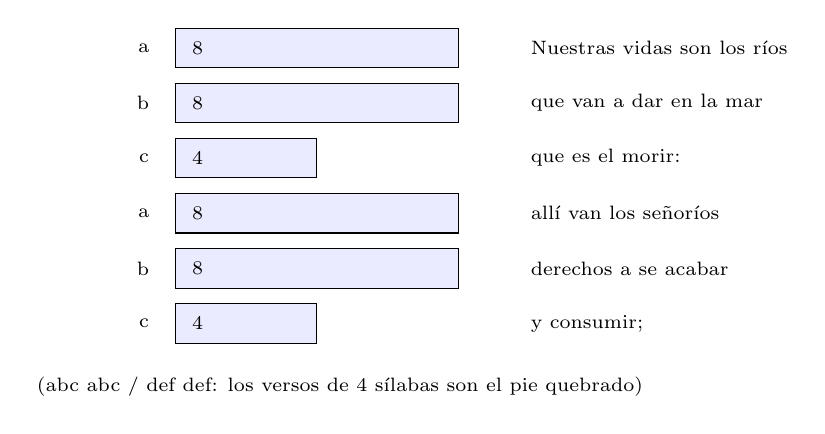
\begin{tikzpicture}

\foreach \l/\y/\s/\t in {a/5.0/8/Nuestras vidas son los ríos,b/4.3/8/que van a dar en la mar,c/3.6/4/que es el morir:,a/2.9/8/allí van los señoríos,b/2.2/8/derechos a se acabar,c/1.5/4/y consumir;} {
  \node[font=\scriptsize, anchor=east] at (0.6,\y) {\l};
  \node[draw, fill=blue!8, minimum height=0.5cm, minimum width={0.45cm*\s}, anchor=west] at (0.8,\y) {};
  \node[font=\scriptsize, anchor=west] at (5.2,\y) {\t};
  \node[font=\scriptsize, anchor=west] at (0.9,\y) {\s};
}
\node[font=\scriptsize, align=center] at (2.9,0.7) {(abc abc / def def: los versos de 4 sílabas son el pie quebrado)};

\end{tikzpicture}
\end{document}
